% !TEX TS-program = pdflatex
% !TEX encoding = UTF-8 Unicode

% This is a simple template for a LaTeX document using the "article" class.
% See "book", "report", "letter" for other types of document.

\documentclass[10pt]{article} % use larger type; default would be 10pt
\usepackage{amsmath , amssymb , amsthm}
\usepackage[table]{xcolor}
\usepackage{circuitikz}
\usepackage{subcaption}
\usepackage{tikz}
\usetikzlibrary{automata, positioning, arrows}
\usepackage{placeins}
\usepackage{centernot}
\usepackage{caption}
\usepackage{subcaption}
\usepackage{qtree}
\usepackage{latexsym}
%\usepackage[utf8]{inputenc} % set input encoding (not needed with XeLaTeX)

\usepackage{geometry} % to change the page dimensions
\geometry{a4paper} % or letterpaper (US) or a5paper or....
 \geometry{margin=3cm} % for example, change the margins to 2 inches all round

\renewcommand{\thesubsection}{\thesection.\alph{subsection}}
\renewcommand{\thesubsubsection}{\thesubsection.\roman{subsubsection}}

\title{Fundamentals of Computing \\
      \Large Coursework 1 \\  MSc Data Science}
\author{Mark Rotchell\\13181875}
\date{}
\begin{document}
\maketitle

\pagebreak
\hspace{0pt}
\vfill
\begin{center}
\section*{Academic Declaration}

I have read and understood the sections of plagiarism in the College Policy on assessment offences and confirm that the work is my own, with the work of others clearly acknowledged. I give my permission to submit my report to the plagiarism testing database that the College is using and test it using plagiarism detection software, search engines or meta-searching software.
\end{center}
\vfill
\hspace{0pt}
\pagebreak
\section{}
\subsection{}
\subsubsection{}
\begin{tabular}{c|c|c||c|c|c}
A & B & C & A $\vee$  B & A $\to$ C & C $\wedge$ $\neg$B\\
\hline
0 & 0 & 0 & 0 & 1 & 0 \\
0 & 0 & 1 & 0 & 1 & 1 \\
0 & 1 & 0 & 1 & 1 & 0 \\
0 & 1 & 1 & 1 & 1 & 0 \\
1 & 0 & 0 & 1 & 0 & 0 \\
\rowcolor[HTML]{CCCCCC}
1 & 0 & 1 & 1 & 1 & 1 \\
1 & 1 & 0 & 1 & 0 & 0 \\
1 & 1 & 1 & 1 & 1 & 0 \\
\end{tabular}

\vspace{20px}
The set is consistent for A=1, B=0 and C=1, as hightlighted in the above truth table
\subsubsection{}
\begin{tabular}{c|c|c||c|c|c}
A & B & C & $\neg$A $\wedge$  $\neg$B &  $\neg$C $\to$ A & $\neg$C $\vee$ B \\
\hline
0 & 0 & 0 & 1 & 0 & 1 \\
0 & 0 & 1 & 1 & 1 & 0 \\
0 & 1 & 0 & 0 & 0 & 1 \\
0 & 1 & 1 & 0 & 1 & 1 \\
1 & 0 & 0 & 0 & 1 & 1 \\
1 & 0 & 1 & 0 & 1 & 0 \\
1 & 1 & 0 & 0 & 1 & 1 \\
1 & 1 & 1 & 0 & 1 & 1 \\
\end{tabular}
 
\vspace{20px}
The set is not consistent as there exists no set of truth values for ${A, B, C}$ such that all of the formulae in the set are true

\subsection{}

\begin{tabular}{c|c|c||c|c|c|c}
A & B & C & $p_1=\neg(A\wedge B)$ & $p_2 = C \to A$ &  $p_3 = C \wedge B$ & $(p_1 \wedge p_2 \wedge p_3) \to C$\\
\hline
0 & 0 & 0 & 1 & 1 & 0 & 1 \\
0 & 0 & 1 & 1 & 0 & 0 & 1 \\
0 & 1 & 0 & 1 & 1 & 0 & 1 \\
0 & 1 & 1 & 1 & 0 & 1 & 1 \\
1 & 0 & 0 & 1 & 1 & 0 & 1 \\
1 & 0 & 1 & 1 & 1 & 0 & 1 \\
1 & 1 & 0 & 0 & 1 & 0 & 1 \\
1 & 1 & 1 & 0 & 1 & 1 & 1 \\
\end{tabular}

\vspace{20px}
The argument is logically correct. There exist no situations in which all of the premises are true and the conclusion is false.
\section{}
\subsection{}
\begin{tabular}{c|c|c||c|c|c}
A & B & C & $A \to \neg B$ & $C \to A$ & $\neg\left((A \to \neg B)\wedge(C \to A)\right)$\\
\hline
0 & 0 & 0 & 1 & 1 & 0 \\
0 & 0 & 1 & 1 & 0 & 1 \\
0 & 1 & 0 & 1 & 1 & 0 \\
0 & 1 & 1 & 1 & 0 & 1 \\
1 & 0 & 0 & 1 & 1 & 0 \\
1 & 0 & 1 & 1 & 1 & 0 \\
1 & 1 & 0 & 0 & 1 & 1 \\
1 & 1 & 1 & 0 & 1 & 1 \\
\end{tabular}

\vspace{20px}
\subsection{}
\begin{center}
\begin{circuitikz} \draw
(0,4) node (B) {B}
(0,2) node (A) {A}
(0,0) node (C) {C}
(1.5,1.5) node[not port] (notA) {}
(4,3) node[and port] (andAB) {}
(4,1) node[and port] (andAC) {}
(6,2) node[or port] (or) {}
(B) -- (andAB.in 1)
(A) -- (andAB.in 2)
(A) -- (notA.in)
(notA.out) -- (andAC.in 1)
(C) -- (andAC.in 2)
(andAB.out) -- (or.in 1)
(andAC.out) -- (or.in 2);
\end{circuitikz}
\end{center}

\subsection{}
\[
\begin{aligned}
       & \neg ((     A \to  \neg B) \wedge   (     C \to  A)  ) \\
\equiv & \neg ((\neg A \vee \neg B) \wedge   (     C \to  A)  ) \\
\equiv & \neg ((\neg A \vee \neg B) \wedge   (\neg C \vee A)  ) \\
\equiv & \neg ((\neg B \vee \neg A)  \wedge   (\neg C \vee A)  ) \\
\equiv & \neg ((     B \to  \neg A)  \wedge   (\neg C \vee A)  ) \\
\equiv &       \neg(      B \to  \neg A)  \vee \neg(\neg C \vee A) \\
\equiv &       \neg(      B \to  \neg A)  \vee     (C \wedge \neg A) \\
\equiv &           (      B \to  \neg A) \to     (C \wedge \neg A) \\
\end{aligned}
\]

\section{}
\begin{center}
$N = A_2 \cdot 2^2 + A_1 \cdot 2^1 + A_0 \cdot 2^0$\\

\vspace{20px}

\begin{tabular}{c|c|c||c|c|c}
$A_2$ & $A_1$ & $A_0$ & $N<3_{10}$ & $A_1 \wedge A_0$ & $A_2 \downarrow (A_1 \wedge A_0)$\\
\hline
0 & 0 & 0 & 1 & 0 & 1 \\
0 & 0 & 1 & 1 & 0 & 1 \\
0 & 1 & 0 & 1 & 0 & 1 \\
0 & 1 & 1 & 0 & 1 & 0 \\
1 & 0 & 0 & 0 & 0 & 0 \\
1 & 0 & 1 & 0 & 0 & 0 \\
1 & 1 & 0 & 0 & 0 & 0 \\
1 & 1 & 1 & 0 & 1 & 0 \\
\end{tabular}

\vspace{20px}

\begin{circuitikz} \draw
(0,0) node (A2) {$A_2$}
(0,1) node (A1) {$A_1$}
(0,3) node (A0) {$A_0$}
(2,2) node[and port] (and01) {}
(4,1) node[nor port] (nor) {}
(A0) -- (and01.in 1)
(A1) -- (and01.in 2)
(and01.out) -- (nor.in 1)
(A2) -- (nor.in 2)
;
\end{circuitikz}
\end{center}
\section{}
The argument is not correct. With the following propositional variables:
\renewcommand{\labelenumi}{\Alph{enumi}}
\begin{enumerate}
\item : 'Jones did not meet Smith last night'
\item : 'Smith was the murderer'
\item : 'Jones is lying'
\item : 'The murder took place after midnight'
\end{enumerate}
the propositions can be summarized as:
\renewcommand{\labelenumi}{$p_{\arabic{enumi}}$}
\begin{enumerate}
\item $= A \to (B\vee C)$
\item $= \neg B \to (A \wedge D)$
\item $= D \to (B \vee C)$
\end{enumerate}

These propositions can all be true whilst the conclusion is false, as show by the below row from the truth table, therefore the argument is not correct

\vspace{20px}

\begin{tabular}{c|c|c|c||c|c|c}
A & B & C & D & $p_1 = A \to (B\vee C)$ & $p_2= \neg B \to (A \wedge D)$ & $p_3= D \to (B \vee C)$ \\
\hline
\multicolumn{4}{c||}{$\cdots$} & \multicolumn{3}{c}{$\cdots$} \\
1 & 0 & 1 & 1 & 1 & 1 & 1\\
\multicolumn{4}{c||}{$\cdots$} & \multicolumn{3}{c}{$\cdots$} \\
\hline
\end{tabular}
\section{}
\subsection{}

Initial digit is a {\ttfamily 1} therefore number is negative. Finding absolute value via following steps:
\begin {tabbing}
Initial word \hspace{30px} \= {\ttfamily 1100 0001 1011 0000 0000 0000 0000 0000} \\
Invert digits \>   {\ttfamily 0011 1110 0100 1111 1111 1111 1111 1111} \\
Add one \> {\ttfamily \ \ \ \ \ \ \ \ \ \ \ \ \ \ \ \ \ \ \ \ \ \ \ \ \ \ \ \ \ \ \ \ \ \ \ \ \ \ 1}\\
Result \> {\ttfamily 0011 1110 0101 0000 0000 0000 0000 0000} \\
\> $=2^{29}+2^{28}+2^{27}+2^{26}+2^{25}+2^{22}+2^{20}=1,045,430,272_{10}$ 
\end{tabbing}
Therefore the number is $-1,045,430,272_{10}$
\subsection{}
\begin{center}
{\ttfamily 1100 0001 1011 0000 0000 0000 0000 0000}

$=2^{31}+2^{30}+2^{24}+2^{23} + 2^{21} + 2^{20}=3,249,537,024_{10}$
\end{center}
\subsection{}
\begin{center}
{\ttfamily 1 $\Big|$ 100 0001 1 $\Big|$ 011 0000 0000 0000 0000 0000}
\end{center}

Sign bit is {\ttfamily 1}, so $S = 1$.

Exponent bits are {\ttfamily 100 0001 1} $=2^7+2^1+2^0=131$, and the bias is 127, so $E=131-127=4$.

Fraction bits are {\ttfamily 011 000 \ldots}, so $F=1+2^{-2}+2^{-3} = 1\dfrac{3}{8}$

So number is $(-1)^S \cdot F \cdot 2^ E = -1 \cdot 1\dfrac{3}{8} \cdot 2^4 = -22$
\section{}
\subsection{}
First find binary representation of $|-107| = 107$
\[
\begin{aligned}
107 / 2 = 53 \text{ remainder } & \mathtt{1} \\
53 / 2 = 26 \text{ remainder } & \mathtt{1} \\
26 / 2 = 13 \text{ remainder } & \mathtt{0} \\
13 / 2 = 6 \text{ remainder } & \mathtt{1} \\
6 / 2 = 3 \text{ remainder } & \mathtt{0} \\
3 / 2 = 1 \text{ remainder } & \mathtt{1} \\
1 / 2 = 0 \text{ remainder } & \mathtt{1} \\
\end{aligned}
\]
reading updwards $107_{10} = \mathtt{110 1011}_2$, then convert to negative in two's complement via
\begin {tabbing}
Initial word \hspace{30px} \= {\ttfamily 0000 0000 0000 0000 0000 0000 0110 1011} \\
Invert digits \> {\ttfamily 1111 1111 1111 1111 1111 1111 1001 0100} \\
Add one \> {\ttfamily \ \ \ \ \ \ \ \ \ \ \ \ \ \ \ \ \ \ \ \ \ \ \ \ \ \ \ \ \ \ \ \ \ \ \ \ \ \ 1}\\
Result \> {\ttfamily 1111 1111 1111 1111 1111 1111 1001 0101} \\
\end{tabbing}
\subsection{}
\[-107_{10} = -\mathtt{110 \ 1011}_2 = -\mathtt{1.1010 \ 11}_2 \times 2^6\]

So, sign bit is {\ttfamily 1}

Exponent is $6_{10} + 127_{10} = 133_{10} = \mathtt{1000 \ 0101}_2$

Fraction is $10 1011$

And full word is

\[\mathtt{1100 \ 0010 \ 1101 \ 0110 \ 0000 \ 0000 \ 0000 \ 0000}\]
\subsection{}
\[-14.375 = -\left(8 + 4 + 2 + \frac{1}{4} + \frac{1}{8}\right) = -\mathtt{1110.011}_2 = -\mathtt{1.1100 \ 11}_2+2^3\]

So, sign bit is {\ttfamily 1}

Exponent is $3_{10} + 127_{10} = 130_{10} = \mathtt{1000 \ 0010}_2$

Fraction is $1100 \ 11$

And full word is

\[\mathtt{1100 \ 0001 \ 0110 \ 0110 \ 0000 \ 0000 \ 0000 \ 0000}\]

\section{}
\subsection{}
%Question 7 a
\[ f(x) = x+1 \]
\subsection{}
%Question 7 b
\[
  f(x) =
  \begin{cases} 
   \ \dfrac{x}{2} & \text{if} \ x \ \text{is even} \\
   \\
   \ \dfrac{x-1}{2} & \text{if} \ x \ \text{is odd} \\
  \end{cases}
\]
\subsection{}
%Question 7 c
\[
  f(x) =
  \begin{cases} 
   \ x + 2 & \text{if} \ 3 \ \text{divides} \ x \\
   \ x - 1 & \text{if} \ 3 \ \text{does not divide} \ x \\
  \end{cases}
\]
\section{}
%Question 8
\subsection{}
%Question 8 a
Note that $f(2) = (2+1) / (2-2) = 3/0$ is undefined, so $f$ is not a function over the whole real domain as stated in the question. As it is not a function, it cannot be an injective nor surjective function, so \underline{$f$ is not injective (one-to-one)} and \underline{$f$ is not surjective (onto)}. 

However, considering instead $f^\prime:\mathbb{R}^\prime \to \mathbb{R}$, where $\mathbb{R}^\prime = \mathbb{R} \setminus \{2\}$, given by $f^\prime(x)=\dfrac{x+1}{x-2}$.

\paragraph{Injectivity}
Suppose:
\[
  \begin{aligned}
    f^\prime(x) &= f^\prime(y), \quad x,y \in \mathbb{R}^\prime \\
    \dfrac{x+1}{x-2} &= \dfrac{y+1}{y-2}\\
    (x+1)(y-2) &= (y+1)(x-2) \\
    xy + y -2x -2 &= xy +x -2y -2 \\
    y-2x &= x - 2y \\
    y &= x \\
  \end{aligned}
\]
so 
\[
\forall \ x,y \in \mathbb{R}^\prime : f^\prime(x) = f^\prime(y) \implies x = y
\]
therefore \underline{$f^\prime$ is injective (one-to-one)}.

\paragraph{Surjectivity} Let $y = f^\prime(x)$, then
\[
  \begin{aligned}
    f^\prime(x) = \dfrac{x+1}{x-2} & = y \\
    x+1 &= y(x-2)\\
    x+1 &= xy - 2y \\
    x(y - 1) &= 1+2y \\
    \end{aligned}
\]
\[ x = \dfrac{1+2y}{y-1} \]
\[\therefore x \ \text{is undefined for} \ y = 1 \]
\[\therefore \ \nexists \ x \in \mathbb{R}^\prime , \ f^\prime(x) = 1\]
\[\therefore \ \neg \left(\forall y \in \mathbb{R}, \exists x \in \mathbb{R}^\prime, f^\prime(x) = y \right) \]
therefore \underline{$f^\prime$ is not surjective (onto)}.
\subsection{}
%question 8(b)
\paragraph{Injectivity}
\[f(0,1) = 0 = f(1,0)\]
however 
\[(0,1) \neq (1,0)\]
\[\therefore \neg \left(\forall (m,n),(p,q) \in \mathbb{Z} \times \mathbb{Z}: f(m,n) = f(p,q) \implies (m,n) = (p,q) \right)
\]
therefore \underline{$f$ is not injective (one-to-one)}

\paragraph{Surjectivity} Suppose $n=1$ then $f(m,n) = f(m,1) = m + 1 -1 = m$. So, 

\[\forall y \in \mathbb{Z}: f(y,1) = y \]
\[\therefore \ \forall y \in \mathbb{Z}, \ \exists (m,n) \in \mathbb{Z} \times \mathbb{Z}, \ f(m,n) =y \]
therefore \underline{$f$ is surjective (onto)}
\subsection{}
%question 8(c)


\paragraph{Injectivity}
\[f(0,-1) = 0 = f(-1,0)\]
however 
\[(0,-1) \neq (-1,0)\]
\[\therefore \neg \left(\forall (m,n),(p,q) \in \mathbb{Z} \times \mathbb{Z} :f(m,n) = f(p,q) \implies (m,n) = (p,q) \right)
\]
therefore \underline{$f$ is not injective (one-to-one)}


\paragraph{Surjectivity}
\[
  \min(|m| - |n| -1) = 0 - 0 - 1 = -1
\]
\[
  \therefore \nexists (m,n) \in \mathbb{Z} \times \mathbb{Z}, f(m,n) < -1
\]
\[\therefore \neg \left( \forall y \in \mathbb{Z}, \exists (m,n) \in \mathbb{Z} \times \mathbb{Z}, f(m,n) =y \right) \]
therefore \underline{$f$ is not surjective (onto)}


\section{}
%Question 9
\subsection{}
\begin{center}
{\centering
\begin{minipage}[b]{0.4\textwidth}
\centering
\begin{tabular}{c|c c c c} 
    & A & B & C & D\\
    \hline
    A & 1 & 2 & 0 & 1\\
    B & 2 & 0 & 3 & 0\\
    C & 0 & 3 & 1 & 1\\
    D & 1 & 0 & 1 & 0\\
\end{tabular}
\end{minipage}
\hspace{20px}
\centering
\begin{minipage}[c]{0.4\textwidth}
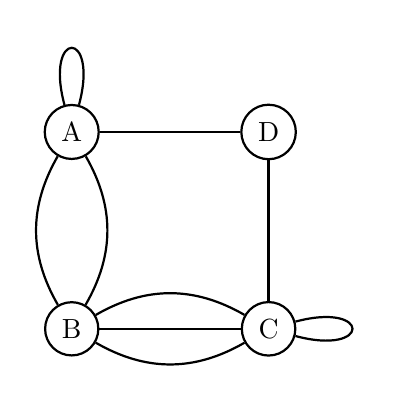
\begin{tikzpicture}[node distance = 2.5cm]
    \begin{scope}[every node/.style={circle,thick,draw}]
        \node (A) {A};
        \node (B) [below of = A] {B};
        \node (C) [right of = B] {C};
        \node (D) [right of = A] {D};
    \end{scope}
    
    \begin{scope}[every edge/.style={draw=black,thick}, every loop/.style={min distance=10mm}]
        \path (A) edge [loop above] (A);
        \path (A) edge [bend right] (B);
        \path (A) edge [bend left]  (B);
        \path (B) edge (C);
        \path (B) edge [bend left]  (C);
        \path (B) edge [bend right] (C);
        \path (C) edge [loop right] (C);
        \path (C) edge (D);
        \path (A) edge (D);
    \end{scope}
\end{tikzpicture}
\end{minipage}}
\end{center}
The graph is not simple as there are vertices with more than one edge between them.
\subsection{}
Let the left hand graph be $G$ such that
\[
	G = (V_G,E_G) = (\{1,2,3,4,5\},\{1,2\},\{1,3\},\{1,5\},\{2,3\},\{2,4\},\{4,5\})
\]
and the right graph be $H$ such that 
\[
	H = (V_H,E_H) = (\{a,c,b,d,e\},\{a,c\},\{a,b\},\{a,e\},\{c,b\},\{c,d\},\{d,e\})
\]
Then let the function $f:V_G\to V_H$ be the vertex bijection given by the following set of pairs of the form $(v,f(v))$:
\[
	\{(1,a),(2,c),(3,b),(4,d),(5,e)\}
\]
Applying the function $f$ to each vertex of each edge $\{v_1,v_2\}$ in $E_G$ gives a set of subsets, ${\{f(v_1),f(v_2)\} \subset V_H}$ which is exactly $E_H$, i.e. all the edges of $H$. 

\vspace{20px}

\begin{tabular}{c|c} 
	$\{v_1,v_2\}$ & $\{f(v_1),f(v_2)\}$ \\
	\hline
	\{1,2\} & \{a,c\} \\
	\{1,3\} & \{a,b\} \\
	\{1,5\} & \{a,e\} \\
	\{2,3\} & \{c,b\} \\
	\{2,4\} & \{c,d\} \\
	\{4,5\} & \{d,e\} \\	
\end{tabular}

\vspace{20px}

All the edges from the two graphs are in above table. No set of vertices which isn't an edge is in the table. If two vertices are adjacent in $G$ their $f$-mapped vertices in $H$ are also adjacent. If two vertices are not adjacent in $G$ their $f$-mapped vertices in $H$ are also not adjacent. Formally

\[
\{v_1,v_2\} \in E_G \iff \{f(v_1),f(v_2)\} \in E_H
\]
therefore $f$ is an isomorphism and $G$ and $H$ are isomorphic.

\subsection{}
The two graphs have a different number of edges, which is an invariant, so the two graphs cannot be isomorphic.
\section{}
\subsection{}

\noindent Computations for $bb$:

\vspace{20px}

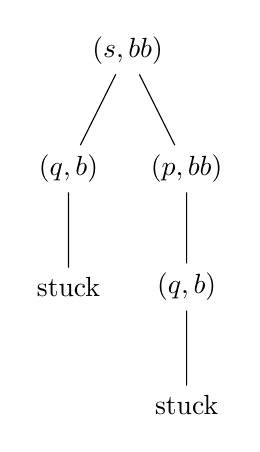
\begin{tikzpicture}[every node/.style = {align=center}]]

 \node {$(s,bb)$}
    child { node {$(q,b)$} 
      child {node {stuck}}
    }
    child { node  {$(p,bb)$}
      child { node {$(q,b)$} 
        child {node {stuck}}
      }
    };
\end{tikzpicture}

\vspace{20px}

\begin{itemize}
  \item $(s,bb), (q,b)$ $\leadsto$ stuck
  \item $(s,bb), (p,bb), (q,b)$  $\leadsto$ stuck
\end{itemize}

\noindent word $bb$ is not accepted

\vspace{20px}

\noindent Computations for $ab$:

\vspace{20px}

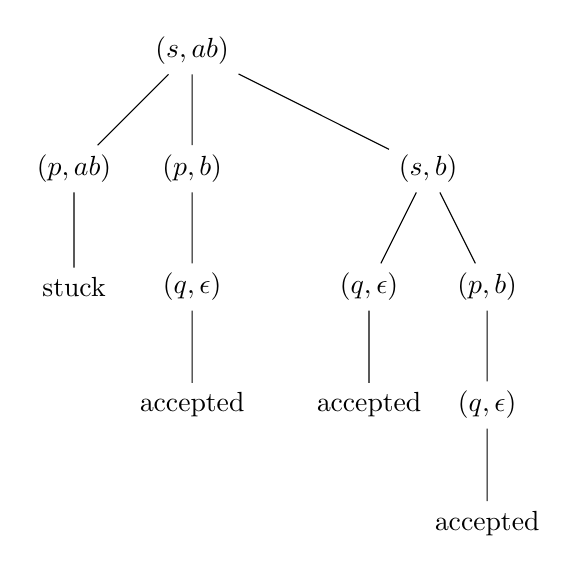
\begin{tikzpicture}[every node/.style = {align=center}]]
 \node {$(s,ab)$}
    child { node {$(p,ab)$} 
      child {node {stuck}}
    }
    child { node {$(p,b)$} 
      child {node {$(q,\epsilon)$}
        child {node {accepted}}
      }
    }
    child { node [right = 1cm] {$(s,b)$} 
      child {node {$(q,\epsilon)$}
        child {node {accepted}}
      }
      child { node {$(p,b)$} 
        child {node {$(q,\epsilon)$}
          child {node {accepted}}
        }
      }
    }
    ;
\end{tikzpicture}

\begin{itemize}
  \item $(s,ab), (p,ab)$ $\leadsto$ stuck
  \item $(s,ab), (p,b), (q,\epsilon)$ $\leadsto$ accepted
  \item $(s,ab), (s,b), (q,\epsilon)$ $\leadsto$ accepted
  \item $(s,ab), (s,b), (p,b), (q,\epsilon)$ $\leadsto$ accepted
\end{itemize}

\noindent word $ab$ is accepted

\vspace{20px}

\noindent Computations for $aba$:

\vspace{20px}
 
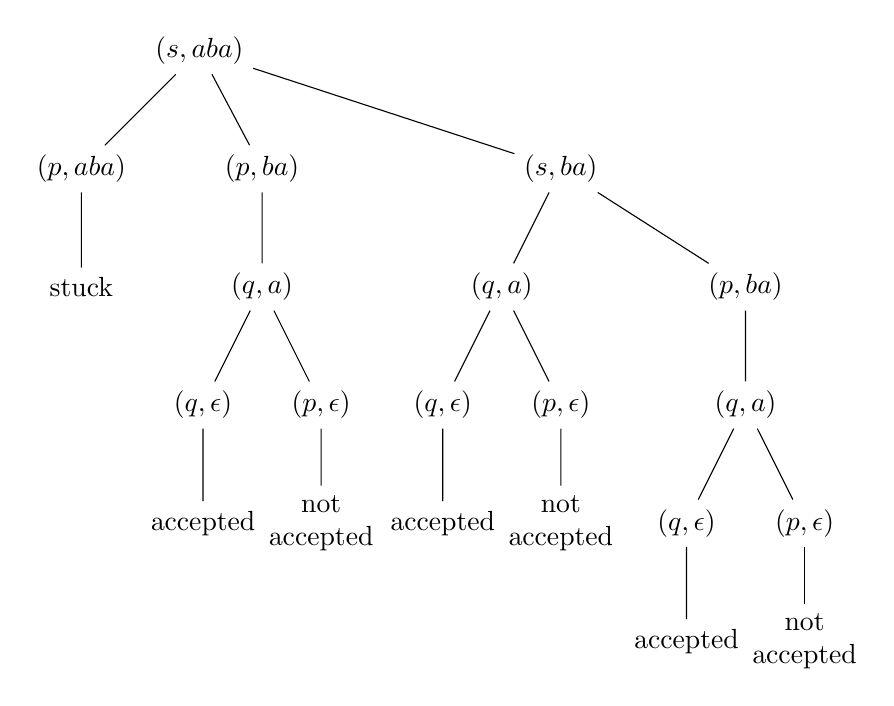
\begin{tikzpicture}[every node/.style = {align=center}]]
 \node {$(s,aba)$}
    child { node {$(p,aba)$} 
      child {node {stuck}}
    }
    child { node [right=2mm] {$(p,ba)$} 
      child {node {$(q,a)$}
        child {node {$(q,\epsilon)$}
          child {node {accepted}}
        }
        child {node {$(p,\epsilon)$}
          child {node {not \\ accepted}}
        }
      }
    }
    child { node [right=25mm] {$(s,ba)$}
      child {node {$(q,a)$}
        child {node {$(q,\epsilon)$}
          child {node {accepted}}
        }
        child {node {$(p,\epsilon)$}
          child {node {not \\ accepted}}
        }
      }
      child {node [right=1cm] {$(p,ba)$}
      child {node {$(q,a)$}
        child {node {$(q,\epsilon)$}
          child {node {accepted}}
        }
        child {node {$(p,\epsilon)$}
          child {node {not \\ accepted}}
        }
      }
      }
    }
    ;
\end{tikzpicture}

\begin{itemize}
  \item $(s,aba), (p,aba)$ $\leadsto$ stuck
  \item $(s,aba), (p,ba), (q,a), (q,\epsilon)$ $\leadsto$ accepted
  \item $(s,aba), (p,ba), (q,a), (p,\epsilon)$ $\leadsto$ not accepted
  \item $(s,aba), (s,ba), (q,a), (q,\epsilon)$ $\leadsto$ accepted
  \item $(s,aba), (s,ba), (q,a), (p,\epsilon)$ $\leadsto$ not accepted
  \item $(s,aba), (s,ba), (p,ba), (q,a), (q,\epsilon)$ $\leadsto$ accepted
  \item $(s,aba), (s,ba), (p,ba), (q,a), (p,\epsilon)$ $\leadsto$ not accepted
\end{itemize}
\noindent word $aba$ is accepted
\subsection{}
\begin{center}
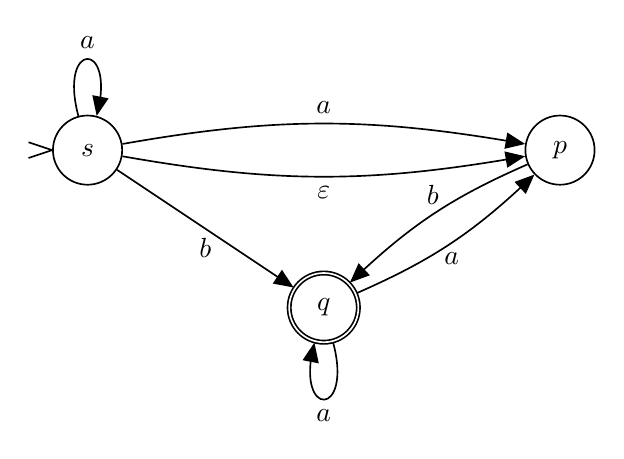
\begin{tikzpicture}[->, 
					>=triangle 45, 
					semithick,
					node distance=2cm, 
					initial text=$ $,
					every loop/.style={min distance=10mm}]

\node[state] (s) at (-3,1) {$s$}; 
\node[state] (p) at (3,1)  {$p$}; 
\node[state, accepting] (q) at (0,-1) {$q$};
\draw 	(s) edge [loop above, above] node{$a$} (s)
		(s) edge [bend left=10, above] node{$a$} (p)
		(s) edge [bend right=10, below] node{$\varepsilon$} (p)
		(s) edge [below] node{$b$} (q)
		(q) edge [bend right = 10, below] node{$a$} (p)
		(p) edge [bend right = 10, above] node{$b$} (q)
		(q) edge [loop below, below] node{$a$} (q);
\draw[-, semithick] (node cs:name=s,anchor=west) -- ++(-3mm,1mm);
\draw[-, semithick] (node cs:name=s,anchor=west) -- ++(-3mm,-1mm);
\end{tikzpicture}
\end{center}

\vspace{20px}

\begin{tabular}{c|c|c}
	subset of states & reachable by $a$ & reachable by $b$ \\
	& followed by one or more  $\varepsilon$ & followed by one or more  $\varepsilon$ \\
	\hline
	$\{s\}$ & $\{s,p\}$ & $\{q\}$\\
	$\{p\}$ & $\O$ &  $\{q\}$\\
	$\{q\}$ & $\{p,q\}$& $\O$ \\
	$\{s,p\}$ & $\{s,p\}$ & $\{q\}$\\
	$\{s,q\}$ & $\{s,p,q\}$ & $\{q\}$\\
	$\{p,q\}$ & $\{p,q\}$ & $\{q\}$\\
	$\{s,p,q\}$ & $\{s,p,q\}$ & $\{q\}$\\
	$\O$ &$\O$  &$\O$  \\
\end{tabular}

\vspace{20px}

The DFA starting state is the $\varepsilon$-closure of the NFA starting state, which is $\{s,p\}$. All subsets with $q$ are accepting states. Full subset construction:

\vspace{20px}

\begin{center}
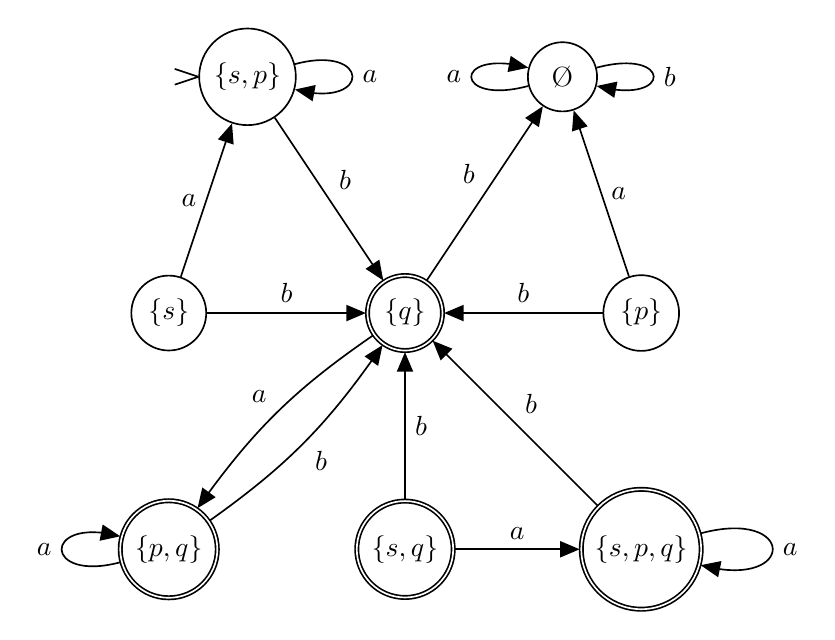
\begin{tikzpicture}[->, 
					>=triangle 45, 
					semithick,
					node distance=2cm, 
					initial text=$ $,
					every loop/.style={min distance=10mm}]

	\node[state] (s) at (-3,0) {$\{s\}$}; 
	\node[state] (p) at (3,0)  {$\{p\}$};
	\node[state, accepting] (q) at (0,0)  {$\{q\}$};
	\node[state] (sp) at (-2,3)  {$\{s,p\}$};
	\node[state, accepting] (sq) at (0,-3)  {$\{s,q\}$};
	\node[state, accepting] (pq) at (-3,-3)  {$\{p,q\}$};
	\node[state, accepting] (spq) at (3,-3)  {$\{s,p,q\}$};
	\node[state] (o) at (2,3)  {$\O$};
	\draw	(s) edge [left] node{$a$} (sp)
			(s) edge [above] node{$b$} (q)
			(p) edge [right] node{$a$} (o)
			(p) edge [above] node{$b$} (q)
			(q) edge [bend right=10, above left] node{$a$} (pq)
			(q) edge [above left] node{$b$} (o)
			(sp) edge [loop right] node{$a$} (sp)
			(sp) edge [above right] node{$b$} (q)
			(sq) edge [above] node{$a$} (spq)
			(sq) edge [right] node{$b$} (q)
			(pq) edge [loop left] node{$a$} (pq)
			(pq) edge [bend right =10, below right] node{$b$} (q)
			(spq) edge [loop right] node{$a$} (sqp)
			(spq) edge [above right] node{$b$} (q)
			(o) edge [loop left] node{$a$} (o)
			(o) edge [loop right] node{$b$} (o)
;
	 
\draw[-, semithick] (node cs:name=sp,anchor=west) -- ++(-3mm,1mm);
\draw[-, semithick] (node cs:name=sp,anchor=west) -- ++(-3mm,-1mm);
\end{tikzpicture}
\end{center}

then removing the unreachable states:

\begin{center}
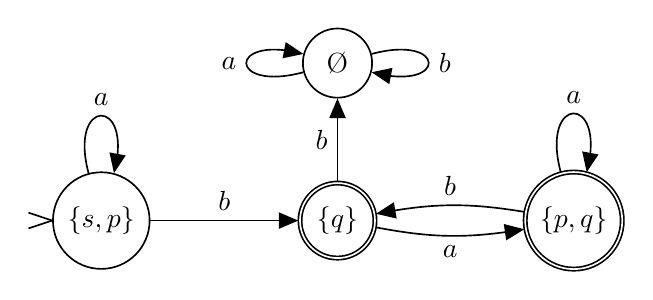
\begin{tikzpicture}[->, 
					>=triangle 45, 
					semithick,
					node distance=2cm, 
					initial text=$ $,
					every loop/.style={min distance=10mm}]

	\node[state, accepting] (q) at (0,0)  {$\{q\}$};
	\node[state] (sp) at (-3,0)  {$\{s,p\}$};
	\node[state, accepting] (pq) at (3,0)  {$\{p,q\}$};
	\node[state] (o) at (0,2)  {$\O$};
	\draw	(q) edge [bend right=10, below] node{$a$} (pq)
			(q) edge [left] node{$b$} (o)
			(sp) edge [loop above] node{$a$} (sp)
			(sp) edge [above] node{$b$} (q)
			(pq) edge [loop above] node{$a$} (pq)
			(pq) edge [bend right =10, above] node{$b$} (q)
			(o) edge [loop left] node{$a$} (o)
			(o) edge [loop right] node{$b$} (o)
;
	 
\draw[-, semithick] (node cs:name=sp,anchor=west) -- ++(-3mm,1mm);
\draw[-, semithick] (node cs:name=sp,anchor=west) -- ++(-3mm,-1mm);
\end{tikzpicture}
\end{center}

then re-labelling the states

\begin{center}
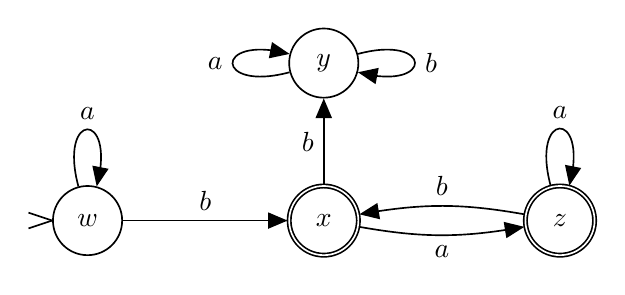
\begin{tikzpicture}[->, 
					>=triangle 45, 
					semithick,
					node distance=2cm, 
					initial text=$ $,
					every loop/.style={min distance=10mm}]

	\node[state, accepting] (q) at (0,0)  {$x$};
	\node[state] (sp) at (-3,0)  {$w$};
	\node[state, accepting] (pq) at (3,0)  {$z$};
	\node[state] (o) at (0,2)  {$y$};
	\draw	(q) edge [bend right=10, below] node{$a$} (pq)
			(q) edge [left] node{$b$} (o)
			(sp) edge [loop above] node{$a$} (sp)
			(sp) edge [above] node{$b$} (q)
			(pq) edge [loop above] node{$a$} (pq)
			(pq) edge [bend right =10, above] node{$b$} (q)
			(o) edge [loop left] node{$a$} (o)
			(o) edge [loop right] node{$b$} (o)
;
	 
\draw[-, semithick] (node cs:name=sp,anchor=west) -- ++(-3mm,1mm);
\draw[-, semithick] (node cs:name=sp,anchor=west) -- ++(-3mm,-1mm);
\end{tikzpicture}
\end{center}

we have a deterministic finite automaton $A=(Q,\Sigma,\delta,q_0,F)$ with
\begin{itemize}
	\item a set of states $Q=\{w, x, y, z\}$
	\item a set of symbols $\Sigma = \{a,b\}$
	\item a transition function $f:Q \times \Sigma \to Q$ given by the below table
	
	\begin{tabular}{c|c c}
		&  \multicolumn{2}{c}{symbol} \\
		state & a & b \\
		\hline
		$w$ & $w$ & $x$ \\
		$x$ & $z$ & $y$ \\
		$y$ & $y$ & $y$ \\
		$z$ & $z$ & $x$ \\
	\end{tabular}
	\item an initial state $q_0 = w$
	\item a set of accepting states $F = \{x, z\}$
\end{itemize}

\subsection{}
The automaton accepts words comprised of $a$ and $b$ that contain at least one $b$, but no consecutive $b$s.
\subsection{}
$\mathtt{a^*b(aa^*b)^*a^*}$
\subsection{}
Let $G=(V,\Sigma,R,s)$ be a context free grammar with
\begin{itemize}
	\item a set of variables $V=\{S,X,Y\}$
	\item a set of terminals $\Sigma = \{a,b\}$
	\item a set of production rules $R = \{S \to XbYX, \ X \to \varepsilon, \ X \to aX, \ Y \to \varepsilon, \ Y \to aXbY\}$
	\item a start variable $s=S$
\end{itemize}
\section{}
Let $A=(Q,\Sigma,\delta,q_0,F)$ be a deterministic finite automaton with
\begin{itemize}
	\item a set of states $Q=\{s,p,q,r\}$
	\item a set of symbols $\Sigma = \{1,0\}$
	\item a transition function $f:Q \times \Sigma \to Q$ given by the below table
	
	\begin{tabular}{c|c c}
		&  \multicolumn{2}{c}{symbol} \\
		state & 0 & 1 \\
		\hline
		$s$ & $p$ & $s$ \\
		$p$ & $q$ & $p$ \\
		$q$ & $q$ & $r$ \\
		$r$ & $q$ & $p$ \\
	\end{tabular}
	\item an initial state $q_0 = s$
	\item a set of accepting states $F = \{q,r\}$
\end{itemize}
We can visualise $A$ with the following state diagram
\begin{center}
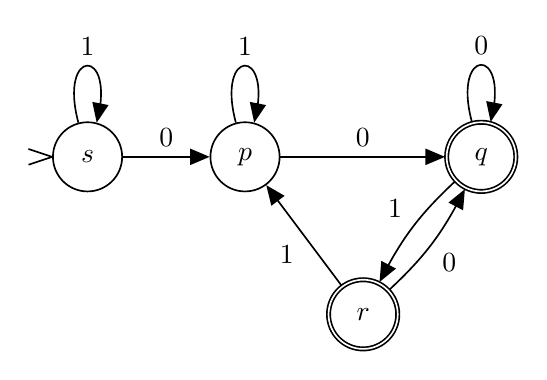
\begin{tikzpicture}[->, 
					>=triangle 45, 
					semithick,
					node distance=2cm, 
					initial text=$ $,
					every loop/.style={min distance=10mm}]

	\node[state] (s) at (-3,0)  {$s$};
	\node[state] (p) at (-1,0)  {$p$};
	\node[state, accepting] (q) at (2,0)   {$q$};
	\node[state, accepting] (r) at (0.5,-2)  {$r$};
	\draw 	(s) edge [loop above] node{$1$} (s)
			(s) edge [above] node{$0$} (p)
			(p) edge [loop above] node{$1$} (p)
			(p) edge [above] node{$0$} (q)
			(q) edge [bend right=10, above left] node{$1$} (r)
			(q) edge [loop above] node{$0$} (q)
			(r) edge [below left] node{$1$} (p)
			(r) edge [below right, bend right=10] node{$0$} (q)
	;
	\draw[-, semithick] (node cs:name=s,anchor=west) -- ++(-3mm,1mm);
	\draw[-, semithick] (node cs:name=s,anchor=west) -- ++(-3mm,-1mm);
\end{tikzpicture}
\end{center}
This can be represented by the following regular expression $\mathtt{1^*0(0\cup 1)^*(0\cup 01)}$
\pagebreak
\section{}
\begin{figure}[!htbp]
  \begin{subfigure}[c]{0.3\textwidth}
    \begin{center}
    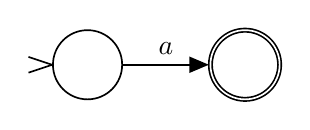
\begin{tikzpicture}[->, >=triangle 45, semithick, node distance=2cm]
    	\node[state] (1) at (-1,0) {};
    	\node[state, accepting] (2) at (1,0)  {};
    	\draw 	(1) edge [above] node{$a$} (2);
    	\draw[-, semithick] (node cs:name=1,anchor=west) -- ++(-3mm,1mm);
    	\draw[-, semithick] (node cs:name=1,anchor=west) -- ++(-3mm,-1mm);
    \end{tikzpicture}
    \end{center}
    \caption*{Automaton accepting $L[a]$}
  \end{subfigure}
  %
  \begin{subfigure}[c]{0.3\textwidth}    
    \begin{center}
    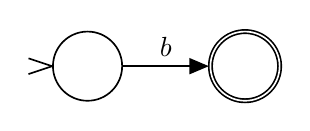
\begin{tikzpicture}[->, >=triangle 45, semithick, node distance=2cm]
    	\node[state] (1) at (-1,0) {};
    	\node[state, accepting] (2) at (1,0)  {};
    	\draw 	(1) edge [above] node{$b$} (2);
    	\draw[-, semithick] (node cs:name=1,anchor=west) -- ++(-3mm,1mm);
    	\draw[-, semithick] (node cs:name=1,anchor=west) -- ++(-3mm,-1mm);
    \end{tikzpicture}
    \end{center}
    \caption*{Automaton accepting $L[b]$}
  \end{subfigure}
  %
  \begin{subfigure}[c]{0.4\textwidth}
    \begin{center}
    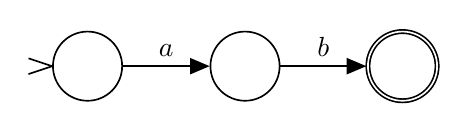
\begin{tikzpicture}[->, >=triangle 45, semithick, node distance=2cm]
    	\node[state] (1) at (-1,0) {};
    	\node[state] (2) at (1,0)  {};
    	\node[state, accepting] (3) at (3,0)  {};
    	\draw 	(1) edge [above] node{$a$} (2)
    	 		(2) edge [above] node{$b$} (3);
    	\draw[-, semithick] (node cs:name=1,anchor=west) -- ++(-3mm,1mm);
    	\draw[-, semithick] (node cs:name=1,anchor=west) -- ++(-3mm,-1mm);
    \end{tikzpicture}
    \end{center}
    \caption*{Automaton accepting $L[ab]$}
  \end{subfigure}
\end{figure}
\begin{figure}[!htbp]
  \begin{subfigure}[c]{0.3\textwidth}
    \begin{center}
    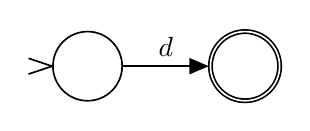
\begin{tikzpicture}[->, >=triangle 45, semithick, node distance=2cm]
    	\node[state] (1) at (-1,0) {};
    	\node[state, accepting] (2) at (1,0)  {};
    	\draw 	(1) edge [above] node{$d$} (2);
    	\draw[-, semithick] (node cs:name=1,anchor=west) -- ++(-3mm,1mm);
    	\draw[-, semithick] (node cs:name=1,anchor=west) -- ++(-3mm,-1mm);
    \end{tikzpicture}
    \end{center}
    \caption*{Automaton accepting $L[d]$}
  \end{subfigure}
  %
  \begin{subfigure}[c]{0.3\textwidth}    
    \begin{center}
    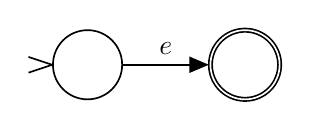
\begin{tikzpicture}[->, >=triangle 45, semithick, node distance=2cm]
    	\node[state] (1) at (-1,0) {};
    	\node[state, accepting] (2) at (1,0)  {};
    	\draw 	(1) edge [above] node{$e$} (2);
    	\draw[-, semithick] (node cs:name=1,anchor=west) -- ++(-3mm,1mm);
    	\draw[-, semithick] (node cs:name=1,anchor=west) -- ++(-3mm,-1mm);
    \end{tikzpicture}
    \end{center}
    \caption*{Automaton accepting $L[e]$}
  \end{subfigure}
  %
  \begin{subfigure}[c]{0.4\textwidth}
    \begin{center}
    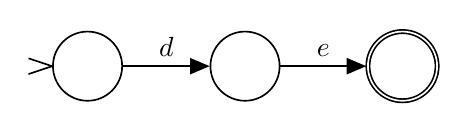
\begin{tikzpicture}[->, >=triangle 45, semithick, node distance=2cm]
    	\node[state] (1) at (-1,0) {};
    	\node[state] (2) at (1,0)  {};
    	\node[state, accepting] (3) at (3,0)  {};
    	\draw 	(1) edge [above] node{$d$} (2)
    	 		(2) edge [above] node{$e$} (3);
    	\draw[-, semithick] (node cs:name=1,anchor=west) -- ++(-3mm,1mm);
    	\draw[-, semithick] (node cs:name=1,anchor=west) -- ++(-3mm,-1mm);
    \end{tikzpicture}
    \end{center}
    \caption*{Automaton accepting $L[de]$}
  \end{subfigure}
\end{figure}
\vspace{20px}
\begin{figure}[!htbp]
  \begin{subfigure}[c]{0.3\textwidth}
    \begin{center}
    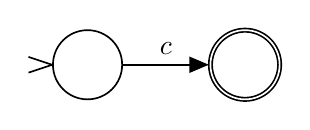
\begin{tikzpicture}[->, >=triangle 45, semithick, node distance=2cm]
    	\node[state] (1) at (-1,0) {};
    	\node[state, accepting] (2) at (1,0)  {};
    	\draw 	(1) edge [above] node{$c$} (2);
    	\draw[-, semithick] (node cs:name=1,anchor=west) -- ++(-3mm,1mm);
    	\draw[-, semithick] (node cs:name=1,anchor=west) -- ++(-3mm,-1mm);
    \end{tikzpicture}
    \end{center}
    \caption*{Automaton accepting $L[c]$}
  \end{subfigure}
  %
  \begin{subfigure}[c]{0.6\textwidth}    
    \begin{center}
    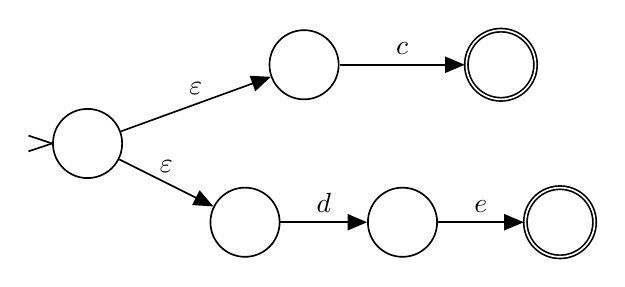
\begin{tikzpicture}[->, >=triangle 45, semithick, node distance=2cm]
    	\node[state] (1) at (-3,0) {};
    	\node[state] (2) at (-0.25,1)  {};
    	\node[state] (3) at (-1,-1)  {};
    	\node[state, accepting] (4) at (2.25,1)  {};
    	\node[state] (5) at (1,-1)  {};
    	\node[state, accepting] (6) at (3,-1)  {};
    	\draw 	(1) edge [above] node{$\varepsilon$} (2)
				(1) edge [above] node{$\varepsilon$} (3)
				(2) edge [above] node{$c$} (4)
				(3) edge [above] node{$d$} (5)
				(5) edge [above] node{$e$} (6)
	;
    	\draw[-, semithick] (node cs:name=1,anchor=west) -- ++(-3mm,1mm);
    	\draw[-, semithick] (node cs:name=1,anchor=west) -- ++(-3mm,-1mm);
    \end{tikzpicture}
    \end{center}
    \caption*{Automaton accepting $L[c\cup de]$}
  \end{subfigure}
\end{figure}
\begin{figure}[!htbp]
  \begin{subfigure}[c]{0.15\textwidth}
    \begin{center}
    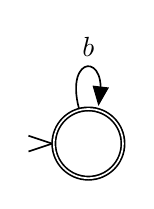
\begin{tikzpicture}[->, >=triangle 45, semithick, node distance=2cm]
    	\node[state, accepting] (1) at (0,0) {};
    	\draw 	(1) edge [loop above] node{$b$} (1);
    	\draw[-, semithick] (node cs:name=1,anchor=west) -- ++(-3mm,1mm);
    	\draw[-, semithick] (node cs:name=1,anchor=west) -- ++(-3mm,-1mm);
    \end{tikzpicture}
    \end{center}
    \caption*{Automaton accepting $L[b^*]$}
  \end{subfigure}
  %
  \begin{subfigure}[c]{0.85\textwidth}    
    \begin{center}
    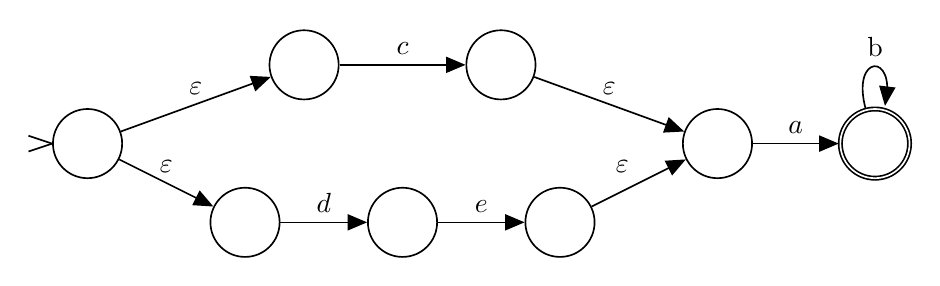
\begin{tikzpicture}[->, >=triangle 45, semithick, node distance=2cm]
    	\node[state] (1) at (-3,0) {};
    	\node[state] (2) at (-0.25,1)  {};
    	\node[state] (3) at (-1,-1)  {};
    	\node[state] (4) at (2.25,1)  {};
    	\node[state] (5) at (1,-1)  {};
    	\node[state] (6) at (3,-1)  {};
    	\node[state] (7) at (5,0)  {};
    	\node[state, accepting] (8) at (7,0)  {};
    	\draw 	(1) edge [above] node{$\varepsilon$} (2)
				(1) edge [above] node{$\varepsilon$} (3)
				(2) edge [above] node{$c$} (4)
				(3) edge [above] node{$d$} (5)
				(5) edge [above] node{$e$} (6)
				(4) edge [above] node{$\varepsilon$} (7)
				(6) edge [above left] node{$\varepsilon$} (7)
				(7) edge [above] node{$a$} (8)
				(8) edge [loop above] node{b} (8)
	;
    	\draw[-, semithick] (node cs:name=1,anchor=west) -- ++(-3mm,1mm);
    	\draw[-, semithick] (node cs:name=1,anchor=west) -- ++(-3mm,-1mm);
    \end{tikzpicture}
    \end{center}
    \caption*{Automaton accepting $L[(c\cup de)ab^*]$}
  \end{subfigure}
\end{figure}
\begin{figure}[!htbp]
  \begin{subfigure}[c]{0.5\textwidth}    
    \begin{center}
    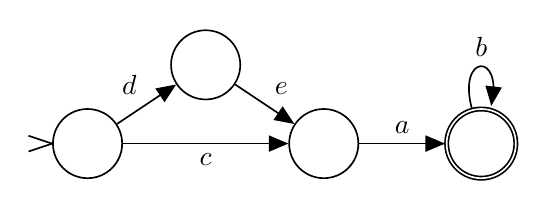
\begin{tikzpicture}[->, >=triangle 45, semithick, node distance=2cm]
    	\node[state] (1) at (-3,0) {};
    	\node[state] (2) at (-1.5,1)  {};
    	\node[state] (3) at (0,0)  {};
    	\node[state, accepting] (4) at (2,0)  {};
    	\draw 	(1) edge [above left] node{$d$} (2)
				(1) edge [below] node{$c$} (3)
				(2) edge [above right] node{$e$} (3)
				(3) edge [above] node{$a$} (4)
				(4) edge [loop above] node{$b$} (4)
	;
    	\draw[-, semithick] (node cs:name=1,anchor=west) -- ++(-3mm,1mm);
    	\draw[-, semithick] (node cs:name=1,anchor=west) -- ++(-3mm,-1mm);
    \end{tikzpicture}
    \end{center}
    \caption*{Simplified Automaton accepting $L[(c\cup de)ab^*]$}
  \end{subfigure}
  \begin{subfigure}[c]{0.5\textwidth}    
    \begin{center}
    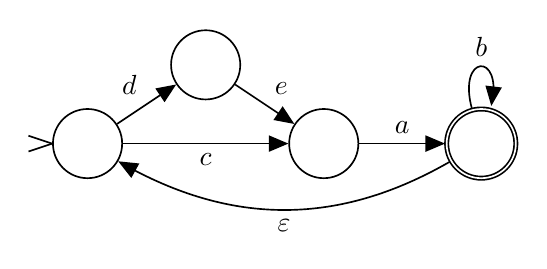
\begin{tikzpicture}[->, >=triangle 45, semithick, node distance=2cm]
    	\node[state] (1) at (-3,0) {};
    	\node[state] (2) at (-1.5,1)  {};
    	\node[state] (3) at (0,0)  {};
    	\node[state, accepting] (4) at (2,0)  {};
    	\draw 	(1) edge [above left] node{$d$} (2)
				(1) edge [below] node{$c$} (3)
				(2) edge [above right] node{$e$} (3)
				(3) edge [above] node{$a$} (4)
				(4) edge [loop above] node{$b$} (4)
				(4) edge [bend left, below] node{$\varepsilon$} (1)
	;
    	\draw[-, semithick] (node cs:name=1,anchor=west) -- ++(-3mm,1mm);
    	\draw[-, semithick] (node cs:name=1,anchor=west) -- ++(-3mm,-1mm);
    \end{tikzpicture}
    \end{center}
    \caption*{Automaton accepting $L[\big(c\cup de)ab^*\big)^*]$}
  \end{subfigure}
\end{figure}
\begin{figure}[!htbp]
  \begin{subfigure}[c]{1\textwidth}    
    \begin{center}
    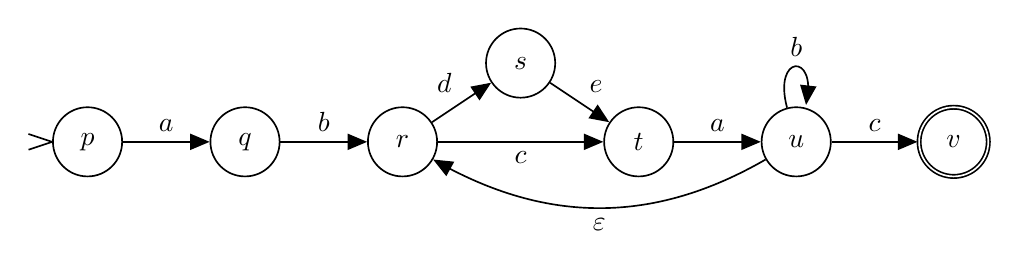
\begin{tikzpicture}[->, >=triangle 45, semithick, node distance=2cm]
    	\node[state] (r) at (-3,0) {$r$};
    	\node[state] (s) at (-1.5,1)  {$s$};
    	\node[state] (t) at (0,0)  {$t$};
    	\node[state] (u) at (2,0)  {$u$};
    	\node[state] (p) at (-7,0)  {$p$};
    	\node[state] (q) at (-5,0)  {$q$};  
    	\node[state,accepting] (v) at (4,0)  {$v$};    	
		\draw 	(r) edge [above left] node{$d$} (s)
				(r) edge [below] node{$c$} (t)
				(s) edge [above right] node{$e$} (t)
				(t) edge [above] node{$a$} (u)
				(u) edge [loop above] node{$b$} (u)
				(u) edge [bend left, below] node{$\varepsilon$} (r)
				(p) edge [above] node{$a$} (q)
				(q) edge [above] node{$b$} (r)
				(u) edge [above] node{$c$} (v)
	;
    	\draw[-, semithick] (node cs:name=p,anchor=west) -- ++(-3mm,1mm);
    	\draw[-, semithick] (node cs:name=p,anchor=west) -- ++(-3mm,-1mm);
    \end{tikzpicture}
    \end{center}
    \caption*{Automaton accepting $L[ab\big(c\cup de)ab^*\big)^*c]$}
  \end{subfigure}
\end{figure}

\FloatBarrier

Let $A=(Q,\Sigma,\delta,q_0,F)$ be a nondeterministic finite automaton with $\varepsilon$ moves, comprising
\begin{itemize}
	\item a set of states $Q=\{p,q,r,s,t,u,v\}$
	\item a set of symbols $\Sigma = \{a,b,c,d,e\}$
	\item a transition function $f:Q \times (\Sigma \cup \{\varepsilon \}) \to \mathsf{Pow}(Q)$ given by the below table
	
	\begin{tabular}{c|c c c c c c}
		&  \multicolumn{6}{c}{symbol} \\
		state & $a$ & $b$ & $c$ & $d$ &$e$ & $\varepsilon$ \\
		\hline
		$p$ & $\{q\}$ & $\varnothing$ & $\varnothing$ & $\varnothing$ & $\varnothing$ & $\varnothing$\\
		$q$ & $\varnothing$ & $\{r\}$ & $\varnothing$ & $\varnothing$ & $\varnothing$ & $\varnothing$\\
		$r$ & $\varnothing$ & $\varnothing$ & $\{t\}$ & $\{s\}$ & $\varnothing$ & $\varnothing$\\
		$s$ & $\varnothing$ & $\varnothing$ & $\varnothing$ & $\varnothing$ & $\{t\}$ & $\varnothing$\\
		$t$ & $\{u\}$ & $\varnothing$ & $\varnothing$ & $\varnothing$ & $\varnothing$ & $\varnothing$\\
		$u$ & $\varnothing$ & $\{u\}$ & $\{v\}$ & $\varnothing$ & $\varnothing$ & $\{r\}$\\
		$v$ & $\varnothing$ & $\varnothing$ & $\varnothing$ & $\varnothing$ & $\varnothing$ & $\varnothing$\\
	\end{tabular}
	\item an initial state $q_0 = p$
	\item a set of accepting states $F = \{v\}$
\end{itemize}
Then $A$ accepts the language $L[ab\big(c\cup de)ab^*\big)^*c]$.
\section{}
\subsection{}
$\mathtt{aaa^*ba^*}$
\subsection{}
$L = \{a^n b^m a^n|n\geq0,m\geq3\}$

\vspace{10px}

$L$ is not regular. Consider words of the form $a^nbbba^n$ which are all in $L$ and can be of any length greater than 3 -- no substring can be removed from these words whilst they remain in $L$: if the substring contains any $b$, and that substring is removed, there will be fewer than 3 $b$; if the substring contains only $a$, and that substring is removed, there will different numbers of $a$ on each side. As there is no substring that can be removed, there is no substring that can be pumped. Therefore, for any length greater than 3 there is a word in $L$ which does not satisfy the pumping property, therefore it is not regular.

\section{}
Let $G=(V,\Sigma,R,s)$ be a context free grammar with
\begin{itemize}
	\item a set of variables $V=\{S,X,Y\}$
	\item a set of terminals $\Sigma = \{a,b,c\}$
	\item a set of production rules $R = \{S \to XY, \ X \to \varepsilon, \ X \to aXb, \ Y \to \varepsilon, \ Y \to bYc\}$
	\item a start variable $s=S$
\end{itemize}

\vspace{20px}

\noindent This would be accepted by a push-down automaton, $P=(Q,\Sigma,\Gamma,\delta,s_0,F)$ with
\begin{itemize}
	\item a set of states, $Q=\{p,q,r,s,t,u\}$
	\item an input alphabet, $\Sigma=\{a,b,c\}$
	\item a stack alphabet, $\Gamma=\{\bot,a,b\}$
	\item a transition relation, $\delta$, consisting of the following instructions of the form ${((q_0,\sigma,\gamma_0),(q_1,\gamma_1))}$
	\begin{itemize}
		\item $((p,\varepsilon,\varepsilon),(q,\bot))$
		\item $((q,a,\varepsilon),(q,a))$
		\item $((q,\varepsilon,\varepsilon),(r,\varepsilon))$
		\item $((r,b,a),(r,\varepsilon))$
		\item $((r,\varepsilon,\bot),(s,\bot))$
		\item $((s,b,\varepsilon),(s,b))$
		\item $((s,\varepsilon,\varepsilon),(t,\varepsilon))$
		\item $((t,c,b),(t,\varepsilon))$
		\item $((t,\varepsilon,\bot),(u,\varepsilon))$
	\end{itemize} where
	\begin{itemize}
		\item $q_0 \in Q$ is the starting state of the transition
		\item $\sigma \in (\Sigma \cup \{\varepsilon\})$ is the input symbol read during the transition
		\item $\gamma_0 \in (\Gamma \cup \{\varepsilon\})$ is the symbol popped from the stack during the transition
		\item $q_1 \in Q$ is the ending state of the transition
		\item $\gamma_1 \in (\Gamma \cup \{\varepsilon\})$ is the symbol pushed onto the stack during the transition
	\end{itemize}
	\item an initial state, $s_0=p$
	\item a set of accepting states $F=\{u\}$
\end{itemize}

\vspace{20px}

\noindent $P$ can be represented by the following state diagram:

\begin{center}
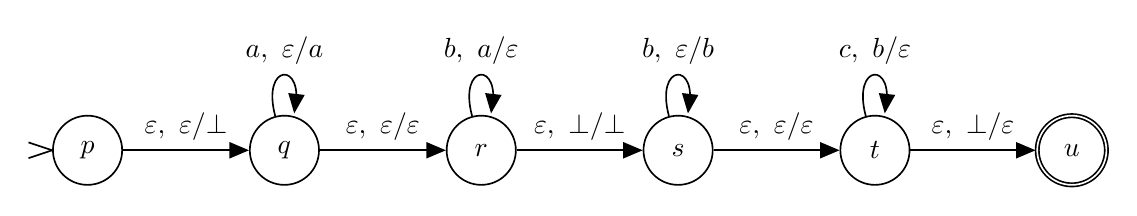
\begin{tikzpicture}[->, >=triangle 45, semithick, node distance=2cm]
	\node[state] (1) at (0,0)  {$p$};
	\node[state] (2) at (2.5,0)  {$q$};
	\node[state] (3) at (5,0)  {$r$};
	\node[state] (4) at (7.5,0)  {$s$};
	\node[state] (5) at (10,0)  {$t$};
	\node[state, accepting] (6) at (12.5,0)  {$u$};
		
		\draw 	(1) edge [above] node{$\varepsilon, \ \varepsilon /\bot$} (2)
				(2) edge [loop above] node{$a, \ \varepsilon / a$} (2)
				(2) edge [above] node{$\varepsilon, \ \varepsilon /\varepsilon$} (3)
				(3) edge [loop above] node{$b, \ a / \varepsilon$} (3)
				(3) edge [above] node{$\varepsilon, \ \bot /\bot$} (4)
				(4) edge [loop above] node{$b, \ \varepsilon / b$} (4)
				(4) edge [above] node{$\varepsilon, \ \varepsilon /\varepsilon$} (5)
				(5) edge [loop above] node{$c, \ b / \varepsilon$} (5)
				(5) edge [above] node{$\varepsilon, \ \bot /\varepsilon$} (6)
		;
	
		\draw[-, semithick] (node cs:name=1,anchor=west) -- ++(-3mm,1mm);
	\draw[-, semithick] (node cs:name=1,anchor=west) -- ++(-3mm,-1mm);
\end{tikzpicture}
\end{center}
\end{document}










